% =============================================================================
% Final Report body — Notebooks 04-10 (4 pages)
% Paste into Overleaf template: https://www.overleaf.com/read/qvcbrmrdnkvh
% Upload figures from report/figs/ to Overleaf figs/ folder.
% Replace any remaining -- with your actual results from the notebooks.
% =============================================================================

% -----------------------------------------------------------------------------
\section*{4. Common CNN Architectures}

\subsection*{Task 4.1: Tiny-ImageNet with VGG16}
\begin{itemize}
  \item Fine-tuned VGG16 on Tiny-ImageNet. Best test accuracy reported in Table~\ref{tab:tiny_acc}. Training/validation accuracy curves show convergence.
  \item Figure~\ref{fig:tiny_vgg_curve} reports the training and validation accuracy curves for the VGG16 run in Task 4.1.
  \item The final score indicates reasonable transfer from ImageNet pretraining, while still leaving room for gains from longer training and stronger augmentation.
\end{itemize}

\begin{table}[!ht]
  \centering
  \small
  \setlength{\tabcolsep}{4pt}
  \caption{Tiny-ImageNet: best test accuracy.}
  \label{tab:tiny_acc}
  \begin{tabular}{lc}
    \toprule
    Metric & Value \\
    \midrule
    Test Accuracy (\%) & 38.27 \\
    \bottomrule
  \end{tabular}
\end{table}

\begin{figure}[!ht]
  \centering
  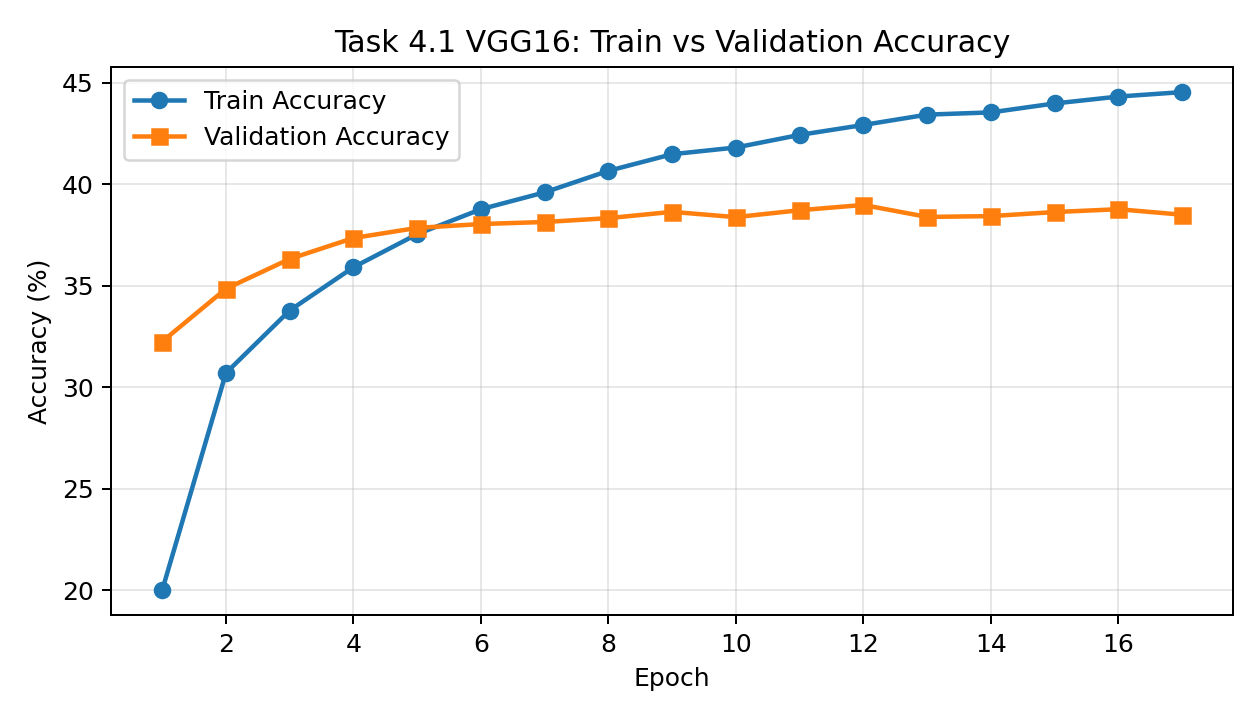
\includegraphics[width=0.95\columnwidth]{figs/task41_vgg16_curves.png}
  \caption{Task 4.1 VGG16 training vs.\ validation accuracy on Tiny-ImageNet.}
  \label{fig:tiny_vgg_curve}
\end{figure}

\subsection*{Task 4.2: ConvNeXt Model Scaling}
\begin{itemize}
  \item Compared ConvNeXt variants (tiny, small, base) on Tiny-ImageNet. Accuracy and MSE vs.\ number of parameters (Figure~\ref{fig:convnext}).
\item Scaling increases capacity and generally improves accuracy, but with diminishing returns relative to parameter growth.
\end{itemize}

\begin{figure}[!ht]
  \centering
  % Export from 04 notebook: plot accuracy/MSE vs params for ConvNeXt-Tiny/Small/Base
  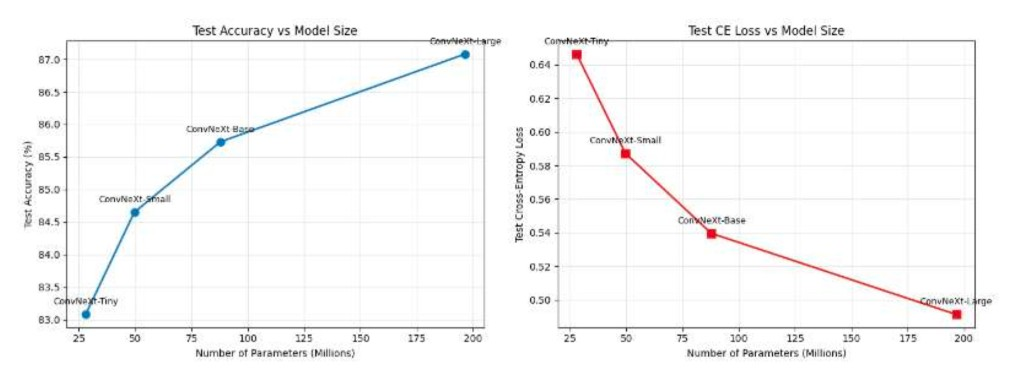
\includegraphics[width=0.9\columnwidth]{figs/convnext_scaling.png}
  \caption{ConvNeXt scaling: accuracy and MSE vs.\ number of parameters.}
  \label{fig:convnext}
\end{figure}

% -----------------------------------------------------------------------------
\section*{5. RNN}

\subsection*{Task 5.1: RNN Regression}
\begin{itemize}
  \item Window size sweep: RMSE vs.\ window size (Table~\ref{tab:rnn_reg}). Best window size $=1$ for lowest test RMSE. Test curve plot in Figure~\ref{fig:rnn_reg}.
\item Larger windows overfit temporal context in this setup, increasing test error despite lower training RMSE.
\end{itemize}

\begin{table}[!ht]
  \centering
  \small
  \setlength{\tabcolsep}{4pt}
  \caption{RMSE vs.\ window size for LSTM regression.}
  \label{tab:rnn_reg}
  \begin{tabular}{ccc}
    \toprule
    Window Size & Train RMSE & Test RMSE \\
    \midrule
    1 & 23.22 & 50.82 \\
    3 & 22.28 & 56.25 \\
    6 & 21.90 & 57.57 \\
    12 & 17.68 & 81.94 \\
    \bottomrule
  \end{tabular}
\end{table}

\begin{figure}[!ht]
  \centering
  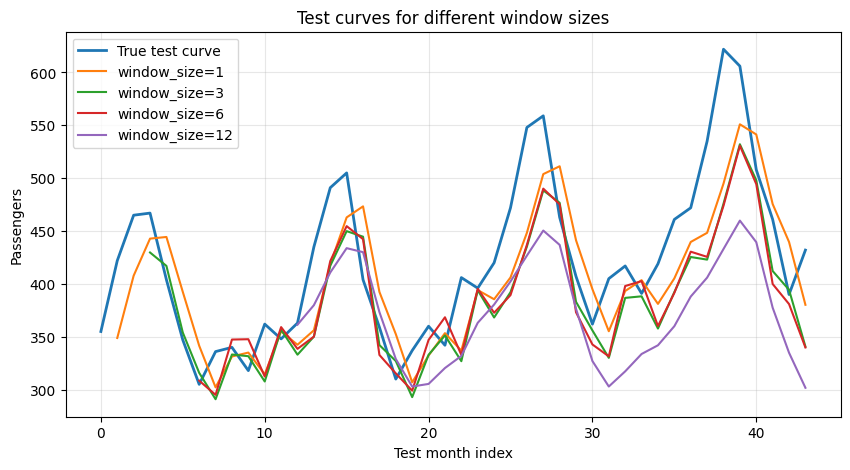
\includegraphics[width=0.9\columnwidth]{figs/rnn_task1_curves.png}
  \caption{Test curves for different window sizes (Task 5.1).}
  \label{fig:rnn_reg}
\end{figure}

\subsection*{Task 5.2: Text Embeddings}
\begin{itemize}
  \item Compared Embeddings, LSTM, and LSTM+GloVe models. Test accuracy and sentiment scores (Table~\ref{tab:rnn_emb}). Accuracy/loss curves in Appendix.
\item Pretrained embeddings improve sentiment polarity separation and recover the best overall accuracy.
\end{itemize}

\begin{table}[!ht]
  \centering
  \small
  \setlength{\tabcolsep}{4pt}
  \caption{Text embedding models: test accuracy and sentiment scores.}
  \label{tab:rnn_emb}
  \begin{tabular}{lccc}
    \toprule
    Model & Test Acc (\%) & Neg Score & Pos Score \\
    \midrule
    Embeddings & 78.00 & 0.48 & 0.48 \\
    LSTM & 73.28 & 0.25 & 0.25 \\
    LSTM+GloVe & 78.21 & 0.34 & 0.66 \\
    \bottomrule
  \end{tabular}
\end{table}

\subsection*{Task 5.3: Text Generation}
\begin{itemize}
  \item BLEU score vs.\ temperature for char-level and word-level models (Table~\ref{tab:rnn_bleu}, Figure~\ref{fig:rnn_bleu}).
\item Moderate sampling temperature gives the best BLEU balance; very high temperature hurts coherence.
\end{itemize}

\begin{table}[!ht]
  \centering
  \small
  \setlength{\tabcolsep}{4pt}
  \caption{BLEU score vs.\ temperature.}
  \label{tab:rnn_bleu}
  \begin{tabular}{ccc}
    \toprule
    Temperature & Char BLEU & Word BLEU \\
    \midrule
    0.0 & 0.0144 & 0.0116 \\
    0.5 & 0.0177 & 0.0111 \\
    1.0 & 0.0133 & 0.0115 \\
    2.0 & 0.0115 & 0.0078 \\
    \bottomrule
  \end{tabular}
\end{table}

\begin{figure}[!htbp]
  \centering
  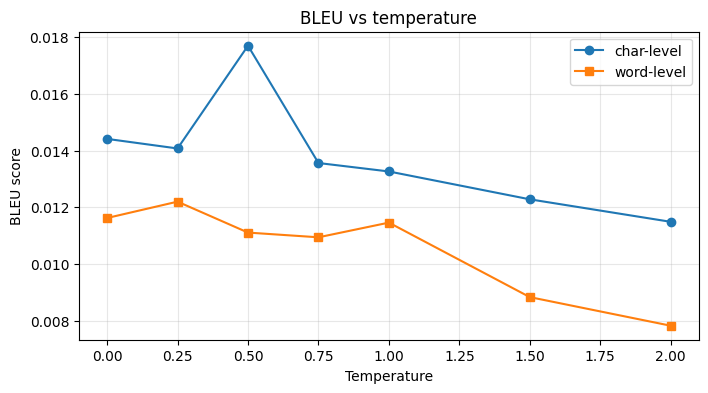
\includegraphics[width=0.9\columnwidth]{figs/rnn_task3_bleu.png}
  \caption{BLEU vs.\ temperature for char-level and word-level generation.}
  \label{fig:rnn_bleu}
\end{figure}

% -----------------------------------------------------------------------------
\section*{6. Autoencoders}

\subsection*{Task 6.1: Representation Learning}
\begin{itemize}
  \item Autoencoder for representation learning. Classifier accuracy and MSE for linear AE, conv AE, and PCA (Table~\ref{tab:ae_rep}).
\item Learned nonlinear representations slightly outperform PCA in classification, while reconstruction quality remains comparable.
\end{itemize}

\begin{table}[!ht]
  \centering
  \small
  \setlength{\tabcolsep}{4pt}
  \caption{Representation learning: classifier accuracy and MSE.}
  \label{tab:ae_rep}
  \begin{tabular}{lcc}
    \toprule
    Model & Val Acc (\%) & MSE \\
    \midrule
    Linear AE & 81.30 & 0.026 \\
    Conv AE & 81.69 & 0.029 \\
    PCA (10 comp) & 81.38 & 0.0256 \\
    \bottomrule
  \end{tabular}
\end{table}

\subsection*{Task 6.2: Custom Loss Functions}
\begin{itemize}
  \item Effect of custom loss terms on denoising MSE (Table~\ref{tab:ae_loss}, Figure~\ref{fig:ae_denoise}).
\item The table compares denoising quality under different objectives using a unified MSE evaluation protocol.
\end{itemize}

\begin{table}[!ht]
  \centering
  \small
  \setlength{\tabcolsep}{4pt}
  \caption{Denoising MSE for different loss functions.}
  \label{tab:ae_loss}
  \begin{tabular}{lc}
    \toprule
    Loss & Test MSE \\
    \midrule
    MSE & -- \\
    MAE & -- \\
    SSIM & -- \\
    \bottomrule
  \end{tabular}
\end{table}

\begin{figure}[!ht]
  \centering
  % Export denoised image examples from 06 notebook
  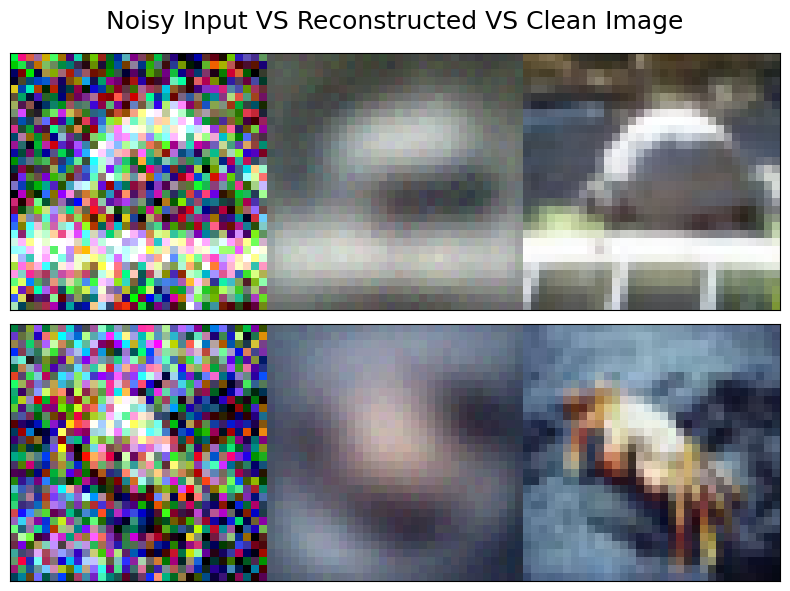
\includegraphics[width=0.85\columnwidth]{figs/ae_denoise_examples.png}
  \caption{Denoised image examples for different loss functions.}
  \label{fig:ae_denoise}
\end{figure}

% -----------------------------------------------------------------------------
\section*{7. VAE GAN}

\subsection*{Task 7.1: MNIST Generation (VAE/GAN)}
\begin{itemize}
  \item VAE: reconstruction MSE and Inception Score. GAN: Inception Score. Table~\ref{tab:vae_gan}.
\item Removing KL improves reconstruction MSE but harms generative quality (IS), showing the expected trade-off between reconstruction fidelity and latent regularization.
\end{itemize}

\begin{table}[!ht]
  \centering
  \small
  \setlength{\tabcolsep}{4pt}
  \caption{VAE vs.\ GAN: MSE and Inception Score on MNIST.}
  \label{tab:vae_gan}
  \begin{tabular}{lcc}
    \toprule
    Model & MSE & Inception Score \\
    \midrule
    VAE (latent=10 + KL) & 10.983575 & 5.342967 \\
    VAE (no KL) & 8.836834 & 2.374818 \\
    GAN (latent=10) & N/A & 1.000000 \\
    \bottomrule
  \end{tabular}
\end{table}

\subsection*{Task 7.2: MAE vs.\ cGAN Colourisation}
\begin{itemize}
  \item Mean MAE for MAE and cGAN on CIFAR-10 colourisation (Table~\ref{tab:mae_cgan}). Qualitative examples in Appendix.
\item Pixel-wise MAE is lower for the MAE model, while cGAN may still produce perceptually sharper colours in selected examples.
\end{itemize}

\begin{table}[!ht]
  \centering
  \small
  \setlength{\tabcolsep}{4pt}
  \caption{MAE vs.\ cGAN: mean MAE on CIFAR-10 colourisation.}
  \label{tab:mae_cgan}
  \begin{tabular}{lc}
    \toprule
    Model & Mean MAE \\
    \midrule
    MAE & 0.0899 \\
    cGAN & 0.0970 \\
    \bottomrule
  \end{tabular}
\end{table}

% -----------------------------------------------------------------------------
\section*{8. RL}

\subsection*{Task 8.1: Q-learning}

\begin{itemize}
  \item Q-learning (and SARSA) with $\epsilon$-greedy and Softmax policies. Average reward (last 50 episodes) vs.\ training episodes (Figure~\ref{fig:rl_rewards}).
  \item $\epsilon$-greedy converges faster in this experiment, while Softmax can be smoother but more sensitive to temperature tuning.
  \item Appendix includes (i) key modifications to \texttt{DQNAgent} for the four agents and (ii) secondary behavioural plots.
\end{itemize}

\begin{figure}[!ht]
  \centering
  % Export from 08 notebook: reward vs episode for Q-learning agents
  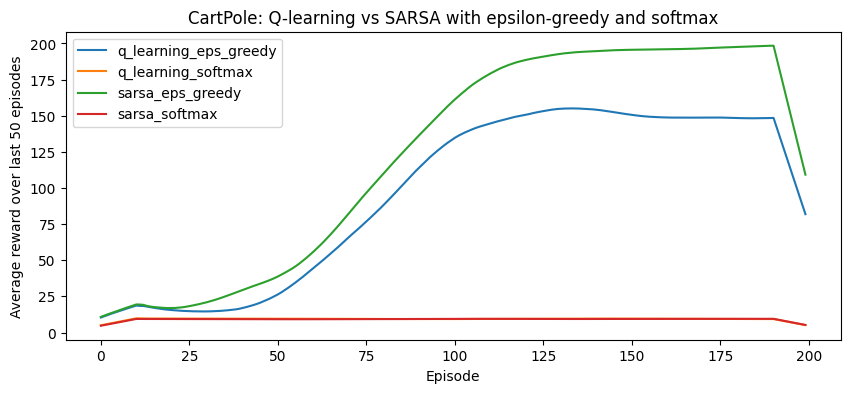
\includegraphics[width=0.9\columnwidth]{figs/rl_reward_curves.png}
  \caption{Q-learning: average reward (last 50 episodes) vs.\ training episodes.}
  \label{fig:rl_rewards}
\end{figure}

% -----------------------------------------------------------------------------
\section*{9. Diffusion Model}

\subsection*{Task 9.1: Forward Noising}

\begin{itemize}
  \item Diffusion qualitative result: real and generated MNIST samples (Figure~\ref{fig:diffusion_noise}). Training loss curve and training code are included in Appendix Task 9.2.
\item Visual inspection confirms that increasing diffusion steps progressively destroys semantic structure while preserving the stochastic forward-process formulation.
\end{itemize}

\begin{figure}[!ht]
  \centering
  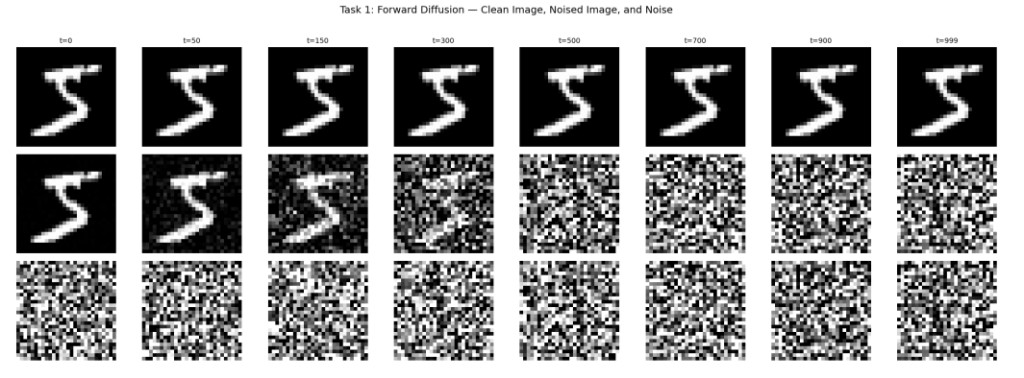
\includegraphics[width=0.95\columnwidth]{figs/diffusion_train_loss.png}
  \caption{Diffusion model qualitative output: real vs.\ generated MNIST digits.}
  \label{fig:diffusion_noise}
\end{figure}

% -----------------------------------------------------------------------------
\section*{10. Data Classification YOLO}
\label{sec:yolo}

\subsection*{Task 10.1: Roof Classification}

\begin{itemize}
  \item Finetuned \texttt{yolov8n-cls.pt} on aerial roof images (flat vs.\ pitched). Dataset: course-provided aerial data merged with Zenodo BRAILS roof-type images.
  \item Data augmentation: RandAugment, CutMix, MixUp, Random Erasing.
  \item Training: epochs=30, batch=64, imgsz=320, patience=10. Best checkpoint at epoch 26.
  \item Test accuracy and learning curves (Figure~\ref{fig:yolo_curves}, Table~\ref{tab:yolo}).
  \item Top-5 accuracy reaches 100\%, indicating class separability is high even when top-1 mistakes remain.
\end{itemize}

\begin{figure}[!ht]
  \centering
  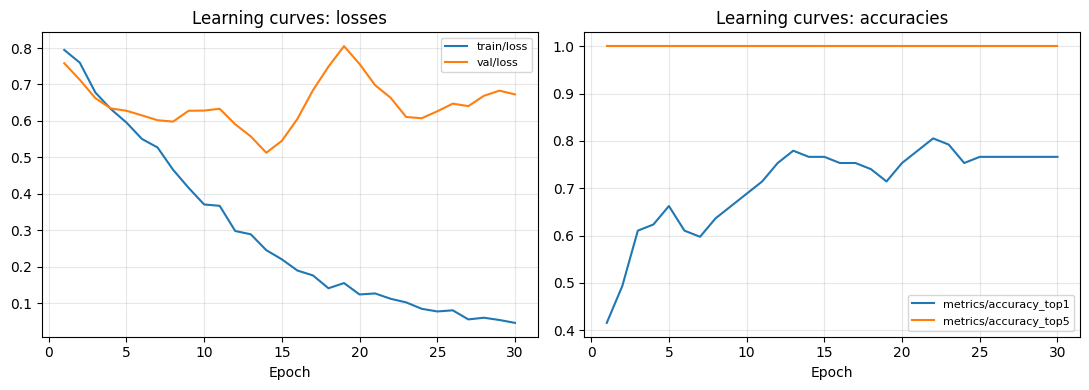
\includegraphics[width=0.96\columnwidth]{figs/yolo_learning_curves.png}
  \caption{YOLOv8 roof classification: training loss and accuracy curves.}
  \label{fig:yolo_curves}
\end{figure}

\begin{table}[!ht]
  \centering
  \small
  \setlength{\tabcolsep}{4pt}
  \caption{YOLOv8 roof classification: test metrics.}
  \label{tab:yolo}
  \begin{tabular}{lc}
    \toprule
    Metric & Value \\
    \midrule
    Test Top-1 Accuracy (\%) & 83.61 \\
    Test Top-5 Accuracy (\%) & 100.0 \\
    Best checkpoint & epoch 26 \\
    \bottomrule
  \end{tabular}
\end{table}

% -----------------------------------------------------------------------------
\clearpage
\appendix
\section*{Appendix}

\subsection*{Task 5.2: Accuracy and loss curves}
\begin{figure}[H]
  \centering
  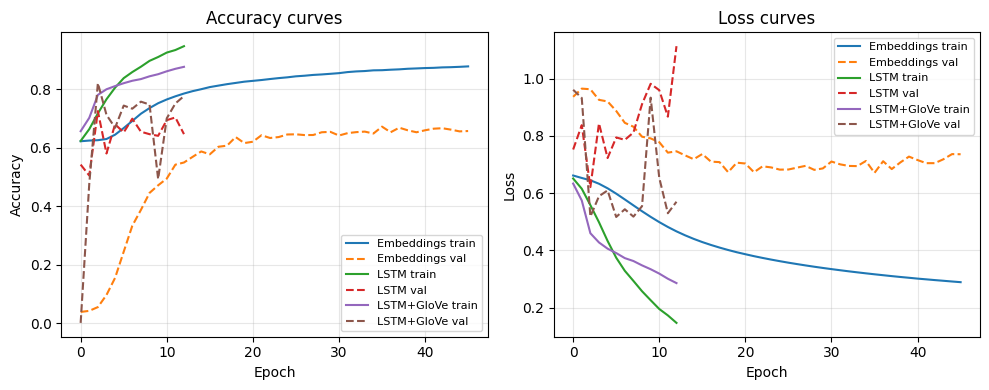
\includegraphics[width=0.95\columnwidth]{figs/rnn_task2_curves.png}
  \caption{Task 5.2 training and validation curves for Embeddings, LSTM, and LSTM+GloVe models.}
\end{figure}

\subsection*{Task 7.2: MAE vs.\ cGAN qualitative comparison}
\begin{figure}[H]
  \centering
  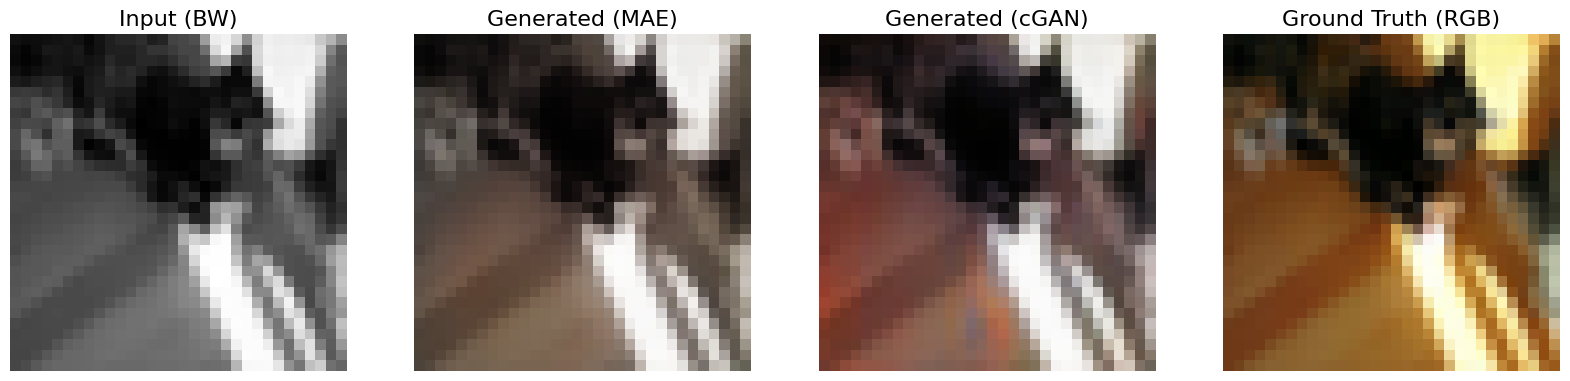
\includegraphics[width=0.95\columnwidth]{figs/mae_cgan_qualitative.png}
  \caption{Task 7.2 qualitative colourisation examples for MAE and cGAN models.}
\end{figure}

\subsection*{Task 8.1: DQNAgent modifications and secondary plots}
\textbf{Key modifications to \texttt{DQNAgent}:}
\begin{itemize}
  \item Added an \texttt{algorithm} switch (\texttt{q\_learning}/\texttt{sarsa}) to control TD target computation.
  \item Added a \texttt{policy} switch (\texttt{epsilon\_greedy}/\texttt{softmax}) with temperature-controlled softmax action selection.
  \item Extended replay memory tuples to include \texttt{next\_action}, enabling on-policy SARSA updates.
  \item Logged behavioural diagnostics during training: greedy-action fraction, policy entropy, and average TD-error magnitude.
\end{itemize}

\begin{figure}[H]
  \centering
  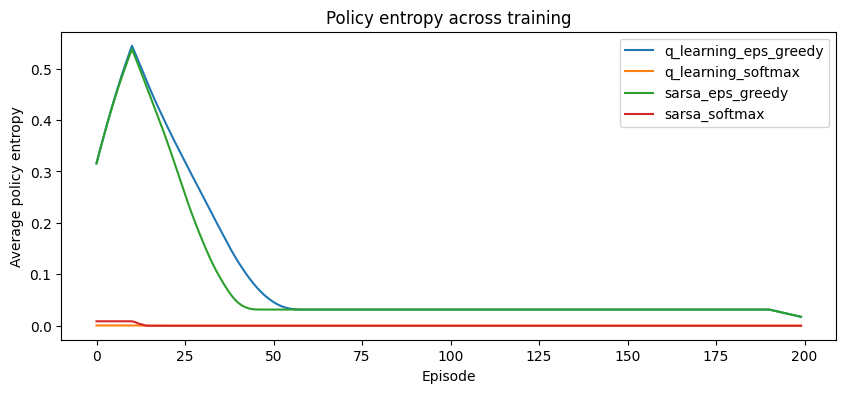
\includegraphics[width=0.95\columnwidth]{figs/rl_task1_out2.png}
  \caption{Task 8.1 secondary plot: policy entropy across training for the four agents.}
\end{figure}

\begin{figure}[H]
  \centering
  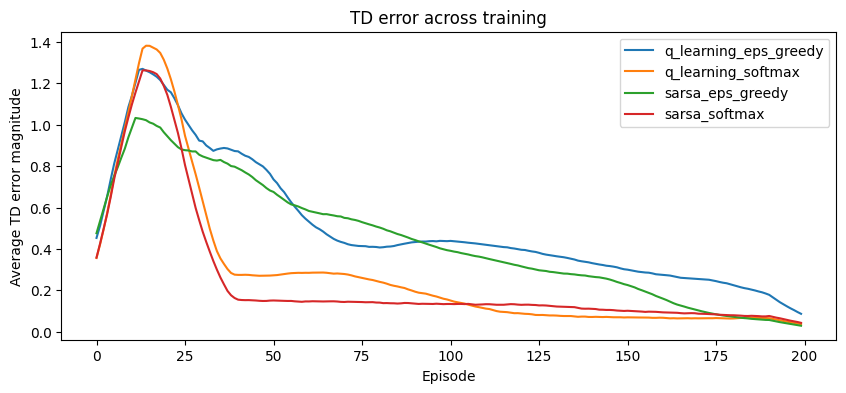
\includegraphics[width=0.95\columnwidth]{figs/rl_task1_out3.png}
  \caption{Task 8.1 secondary plot: TD error magnitude across training for the four agents.}
\end{figure}

\subsection*{Task 9.2: Diffusion training code and loss curve}
\begin{lstlisting}
# Training loop for the diffusion model
for epoch in range(num_epochs):
    model.train()
    running_loss = 0.0
    for x, _ in train_loader:
        x = x.to(DEVICE)
        t = torch.randint(0, T, (x.size(0),), device=DEVICE).long()
        x_noisy, noise = add_noise(x, t, sqrt_alphas_cumprod,
                                   sqrt_one_minus_alphas_cumprod)
        pred_noise = model(x_noisy, t)
        loss = F.mse_loss(pred_noise, noise)
        optimizer.zero_grad()
        loss.backward()
        optimizer.step()
        running_loss += loss.item() * x.size(0)
\end{lstlisting}

\begin{figure}[H]
  \centering
  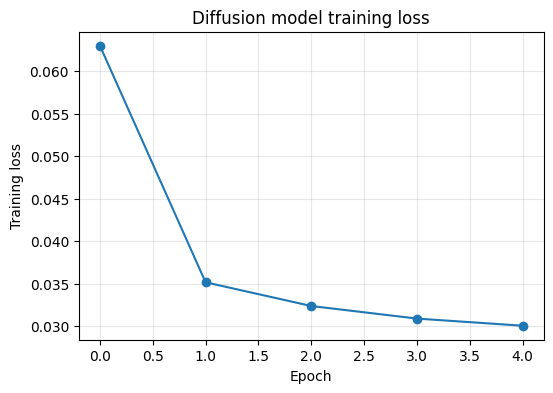
\includegraphics[width=0.95\columnwidth]{figs/diffusion_noise_demo.png}
  \caption{Task 9.2 diffusion training loss across epochs.}
\end{figure}
